\documentclass[a4paper,10pt]{article}
\usepackage[utf8]{inputenc}
\usepackage[style=numeric,backend=biber]{biblatex}
\addbibresource{qrefs.bib}

\newcommand{\yup}{\checkmark}
\newcommand{\nup}{$\times$}
\newcommand{\nyup}{\mbox{$\ket{\times} + \ket{\yup}$}}

\newcommand{\bra}[1]{\langle #1 |}
\newcommand{\ket}[1]{| #1 \rangle}
\newcommand{\braket}[2]{\langle #1 | #2 \rangle}
\newcommand{\ketbra}[2]{| #1 \rangle\langle #2 |}

%opening
\title{Quantum Programming Without Tears}
\author{
Max Cutugno 
\and
Josh Gordon
\and
Tino Tamon
}
\date{\today}

\usepackage{color}
\usepackage{hyperref}
\usepackage{amsmath,amsfonts,amssymb}
\usepackage{graphicx}


\begin{document}

\maketitle

\begin{abstract}
We benchmarked several platforms for quantum computing by running important quantum algorithms on them.
\end{abstract}

\tableofcontents

\section{Platforms}

We tested four platforms.
\begin{enumerate}
\item Liquid
\item PyQuil
\item QISkit
\item Quipper
\end{enumerate}
These have been ordered in increasing difficulty to install. In the interest of reducing future suffering, we have documented our install process for each, as well as provided descriptions of them.
\subsection{Descriptions}
PyQuil and QISkit are very similar; they are both python based, their main purpose is to describe a quantum assembly language, and they come with an API to run your programs on a quantum computer (either at Rigetti Computing with PyQuil or IBM with QISkit). \\
Liquid is Microsoft's platform, and it uses the Q\# language. It comes with a simulator to run circuits, with no option for running on an actual quantum computer. \\
Quipper is an embedded language in Haskell, and is developed by Peter Selinger and Benoit Valiron. It has three simulators, but no option to run programs on a quantum computer.\\
\\
Both PyQuil, Liquid, and Quipper come with a library of quantum algorithms. Liquid has an incomplete version of QLSA, and we have not been able to run the Quipper version.

\subsection{Installation}

\subsubsection{Liquid}

%I actually don't know how you two installed this, so I'm waiting to write it until I can ask

\subsubsection{PyQuil}
To install PyQuil, we used pip. This worked on Windows, however, we found Anaconda to be easier on Mac and Linux.

\begin{quote}
\begin{verbatim}
pip install pyquil
\end{verbatim}
\end{quote}

But, we can also install it within a conda environment as follows:
\begin{quote}
\begin{verbatim} 
$ source activate myquil
(myquil) $ pip install pyquil
(myquil) $ pyquil-config-setup
Welcome to PyQuil!
Enter the required information below for Forest connections.
If you haven't signed up yet you will need to do so first 
  at https://forest.rigetti.com
Forest API Key: <ENTER API HERE>
User ID: <ENTER ID HERE>
Pyquil config file created at '/home/tino/.pyquil_config'
If you experience any problems see the guide 
  at https://go.rigetti.com/getting-started
\end{verbatim}
\end{quote}
Now, we can run some python programs in a directory of examples:
\begin{quote}
\begin{verbatim} 
(myquil) $ python run_quil.py hello_world.quil 
Running Quil Program from:  hello_world.quil
---------------------------
Output: 
[[1, 0, 0, 0, 0, 0, 0, 0]]
\end{verbatim}
\end{quote}

\subsubsection{QISkit}

Installing QISkit was similar; we used pip on windows and Anaconda on Mac and Linux.

\begin{quote}
\begin{verbatim}
pip install qiskit
\end{verbatim}
\end{quote}
It may be helpful to have Jupyter Notebook installed for running some of the examples in QISkit.

\subsubsection{Quipper}

Quipper was the hardest to install, as the package manager for Haskell, Cabal, did not work for some of the dependencies, namely easyrender and newsynth among others.

The key is to download the source for Quipper from the website at \\
\url{https://www.mathstat.dal.ca/~selinger/quipper/}.
Once you have the source, extract it to a folder of your choosing. Use cabal to install as many of the dependencies as you can. Some will fail, but this is no cause for alarm. Simply go to the Haskell package repository, hackage, and download the source for that dependency. Extract the folder with the module you need into your Quipper folder.

\section{Helpful Tools}
\subsection{Anaconda}

To install python in a self-contained environment (which may avoid subtle clashes between python2 
and python3 as well as their respective libraries), one option is to use anaconda. 
We stress that this is optional as one can install pyquil directory without using anaconda.

First, we install anaconda into some directory, say {\tt anaconda2}.
Then, to make it visible globally, we update the bash file {\tt .bashrc}:
\begin{quote}
\begin{verbatim}
#Place the following line in the file .bashrc (at the end)
export PATH="$USER/anaconda2/bin:$PATH"
\end{verbatim}
\end{quote}
Here the variable {\tt \$USER} specifies the path to the user's main directory.
Make sure to source the file from the command line:
\begin{quote}
\begin{verbatim}
$ source .bashrc
\end{verbatim}
\end{quote}
Now conda should be visible from anywhere.

We can update conda first (to catch any latest upgrades):
\begin{quote}
\begin{verbatim}
$ conda update conda
\end{verbatim}
\end{quote}

Now, we create a conda {\em environment} for running our python based programs:
\begin{quote}
\begin{verbatim}
# create a new conda environment called 'myquil'
$ conda create --name myquil python=python3.6
$ conda env list
\end{verbatim}
\end{quote}
To enter the conda environment, we do
\begin{quote}
\begin{verbatim} 
$ source activate myquil
(myquil) $
\end{verbatim}
\end{quote}
and to exit we do
\begin{quote}
\begin{verbatim} 
(myquil) $ source deactivate
$
\end{verbatim}
\end{quote}

\subsection{Jupyter Notebook}

If one wishes to use Jupyter notebook, we need to the add the conda environment
to the notebook. First, we enter the conda environment and then install a python kernel 
for jupyter notebook and connect it to the conda environment:
\begin{quote}
\begin{verbatim} 
(myquil) $ pip install ipykernel
(myquil) $ python -m ipykernel install --user --name myquil
\end{verbatim}
\end{quote}
%Installed kernelspec myquil in <$USER>/.local/share/jupyter/kernels/myquil
Now, we can run jupyter notebook (from outside conda) and choose the appropriate 
kernel (and hence conda environment).


\section{Main algorithms}

We examine several basic known quantum algorithms and verify if they are implemented 
within a certain quantum software platform.

Most of these algorithms are analyzed in \cite{NC00}.

\bigskip

\begin{tabular}{|l||c|c|c|c||} \hline
NAME						& Pyquil& QISkit& Quipper& Liquid \\ \hline \hline
%Bell circuit 				& \yup	& \yup	& \nup	& \nup \\ \hline
teleportation 				& \yup	& \yup	& \yup	& \yup \\ \hline \hline
%Deutsch	 					& \nup	& \nup	& \nup	& \nup \\ \hline
Deutsch-Jozsa				& \yup	& \yup	& \nup	& \nup \\ \hline
Bernstein-Vazirani			& \yup	& \yup	& \nup	& \nup \\ \hline
Simon						& \nup	& \yup	& \nup	& \nup \\ \hline \hline
QFT							& \nup	& \yup	& \yup	& \nup \\ \hline
Phase estimation			& \nup	& \yup	& \nup	& \nup \\ \hline
Shor						& \nup	& \nup	& \nup	& \nup \\ \hline \hline
Grover						& \nup	& \yup	& \yup	& \yup \\ \hline \hline
Amplitude amplification		& \nup	& \yup	& \nup	& \yup \\ \hline \hline
Quantum walk				& \yup	& \yup	& \yup	& \nup \\ \hline \hline
%Singular value estimation	& \nup	& \nup	& \nup	& \nup \\ \hline
Hamiltonian simulation		& \nup	& \nup	& \nup	& \nup \\ \hline
QLSA						& \nup	& \nup	& \nyup	& \nyup \\ \hline \hline
\end{tabular}

\bigskip

\section{Additional algorithms}

\begin{enumerate}
\item (D\"{u}rr and H$\o{}$yer) Finding the minimum element in an array.

\item (Ambainis) Determining if an array contains distinct items.

\item (Child and Goldstone) Continuous-time spatial search.

\end{enumerate}

\section{Cross Compilation}

During testing, we developed several tools for interfacing these platforms. In the interest of not writing the same code many times, most of said tools are translators. \\
The focus of the translators is on a graphical tool for designing circuits we developed. This representation is called Circuit Diagrams.

\begin{center}
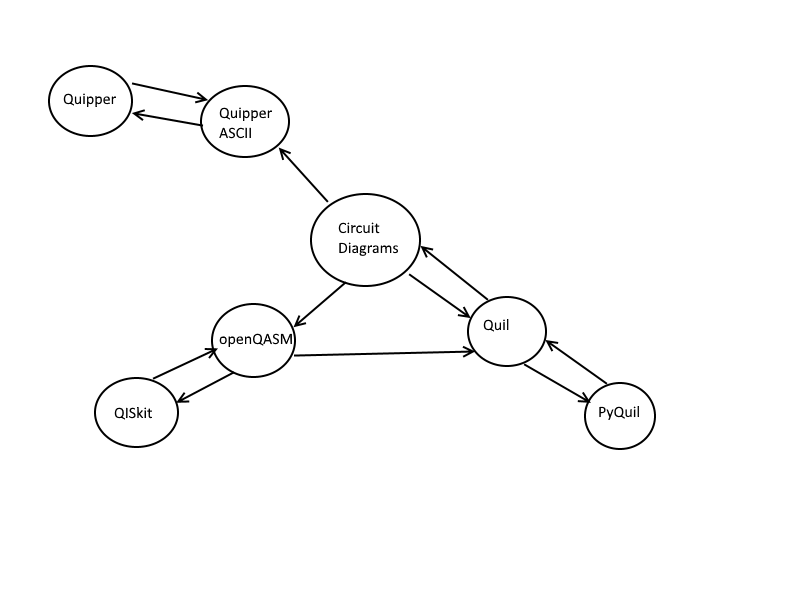
\includegraphics[width=15cm]{translation}
\end{center}


\printbibliography

\end{document}
